\documentclass[a4paper,12pt]{article}
%-----------
\usepackage{lipsum}
\usepackage{amssymb}
\usepackage{amsmath}
\usepackage{graphicx}
\usepackage{placeins}
\usepackage{a4wide}
\usepackage[dutch]{babel}
\usepackage{multicol}
\usepackage[makeroom]{cancel}
\usepackage{enumerate}
\usepackage{epstopdf}
\usepackage{lscape}
%\usepackage{caption}
\usepackage[labelfont=bf]{caption}
\usepackage{hyperref}
%-----------
\usepackage[utf8]{inputenc}
\usepackage[T1]{fontenc}
%-----------
\title{Inleiding Programmeren: \\ Verwerking Examenopdracht}
\date{20-05-2019}
\author{Stoops Tom \\ 2 Ba Fysica}
%-----------
\newcommand{\paf}[2]{\frac{\partial #1}{\partial #2}}
%syntax: \partaf{A}{x} is partiele afgeleide van A naar x geevalueerd in x
\newcommand{\prop}[2]{s_{#2}^2\cdot\left(\paf{#1}{#2}\right)^2}
%syntax: analoog aan partaf, maar dan voor de propagatieformule (enkel sommeren erover en onder een wortel plaatsen: s_x = \sqrt{\prop{A}{a}+\prop{B}{b}+\ldots}
\renewcommand{\thefootnote}{\Roman{footnote}}
%\renewcommand{\phi}{\varphi}
\newcommand{\af}[3]{\frac{d^{#1}#2}{d {#3}^{#1}}}
%syntax: \af{4}{y}{x} is de 4de afgeleide van y naar x, voor 1ste afgeleide de eerste {} gewoon leeg laten!
\newcommand{\ste}{$^\mathrm{ste}\ $}
\newcommand{\de}{$^\mathrm{de}\ $}
%syntax: gewoon achter getal plaatsen
\newcommand{\p}[1]{\left(#1\right)}
\newcommand{\s}[1]{\left[#1\right]}
\newcommand{\avg}[1]{\left\langle#1\right\rangle}
\newcommand{\ta}{$\pm$}
\newcommand{\cirkel}[1]{\raisebox{.5pt}{\textcircled{\raisebox{-1.1pt} {#1}}}}
%-----------
\captionsetup{width=0.8\textwidth}
%-----------
\begin{document}
\pagenumbering{arabic}
\maketitle
\tableofcontents

\newpage
\section{Probleem 1: Superpositie van source-sink pair}
  \noindent
  Voor de eerste opdracht bekeken we de superpositie van een source-sink paar. Voor de configuratie waar de source geplaatst is op $\p{-1,0}$ en sink op $\p{1,0}$ beide met gelijke sterkte $Q$ vinden we de stroomlijnen en snelheidsvectoren zoals weergegeven op figuur \ref{probleem1_1}, wat een zeer intu\"itief resultaat is. Op figuur \ref{probleem1_2} zijn de equipotentiaallijnen weergegeven op een contourplot. Dit komt ook overeen met intu\"itie, op figuur \ref{probleem1_3} zijn de plots samen weergegeven. Op deze figuur kan men duidelijk de relatie tussen snelheidsvectoren en potentiaal vinden zoals gegeven in \cite{opdracht}:

  \begin{equation*}
    \overline{v}\p{x,y} = \overline{\nabla\phi}\p{x,y}
  \end{equation*}

  \noindent
  Waar de snelheidsvector $\overline{v}\p{x,y}$ gegeven is door de gradi\"ent van het potentiaalveld $\phi\p{x,y}$. Dit is ook duidelijk uit de figuur, daar de gradi\"ent het pad van sterkste stijging geeft en dus loodrecht staat op de krommen van gelijke waarde.\\

  \noindent
  Vervolgens is het ook nog interessant om te bekijken wat er gebeurt indien de source en sink verschillende sterktes hebben: $Q_{source} \neq Q_{sink}$, in figuur \ref{probleem1_4} is dit gegeven voor een source die een factor 4 sterker is dan de sink. Ook hier is het resultaat vrij intu\"itief; de source is opmerkelijk sterker dan de sink, waardoor er een deel van de stroomlijnen die vanuit de source vertrekken in de sink terecht komen, maar ook een deel die gewoon aan de sink voorbijlopen.\\

  \noindent
  Tot slot voor deze opdracht bestudeerden we ook nog wat er gebeurde indien de sterktes van de source en sink afhankelijk werden van de afstand tot elkaar:

  \begin{equation*}
    Q\cdot\ell = c^{te} \quad\text{met } Q = Q_{source} = Q_{sink}
  \end{equation*}

  \noindent
  Waar $\ell$ de afstand tussen de source en sink is. We op de verschillende plots van figuur \ref{probleem1_5} dat voor de limiet waar $\ell\rightarrow0$ dat het patroon van stroomlijnen convergeert naar dat van een source-sink doublet zoals gegeven in de opdracht \cite{opdracht}.\\

  \paragraph{Opmerking:} In de code (bijgeleverd in \texttt{.cpp}-formaat) werd er voor source en sink slechts \'e\'en klasse ge\"implementeerd daar we een sink kunnen interpreteren als een source met negatieve sterkte.

  \FloatBarrier
  \begin{figure}[ht!]
    \centering
    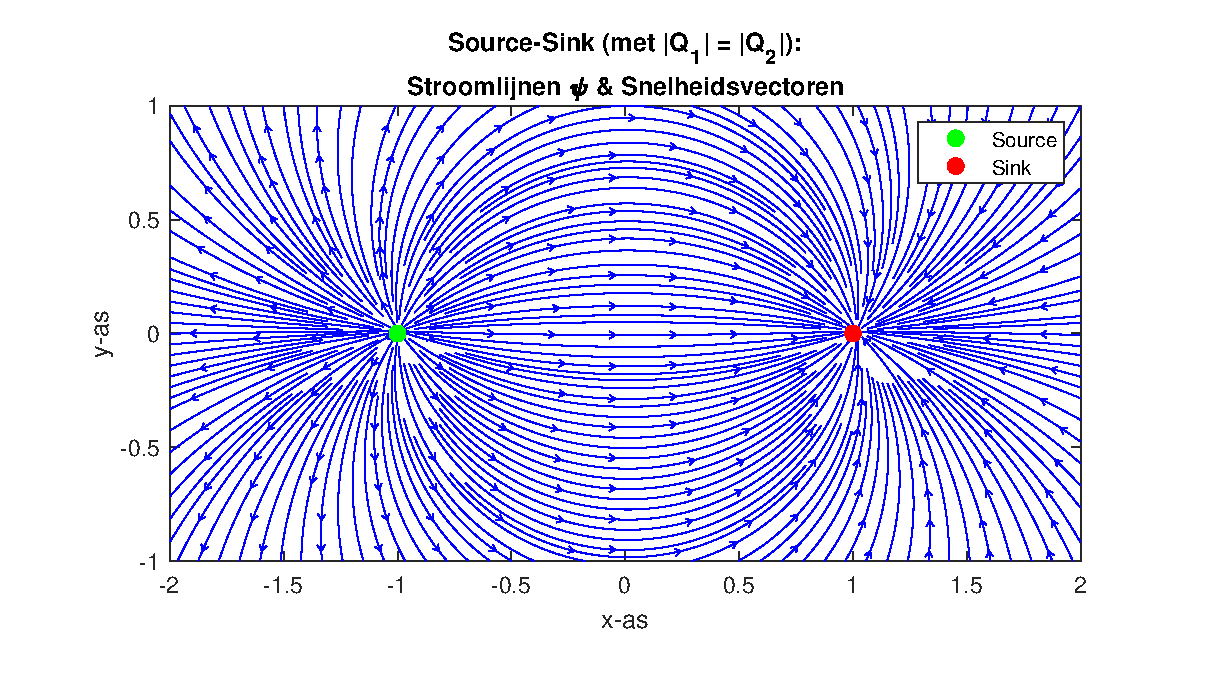
\includegraphics[width = \textwidth]{plots/probleem1_1.eps}
    \caption{Weergave van de stroomlijnen en snelheidsvectoren voor een source-sink paar.}
    \label{probleem1_1}
  \end{figure}
  \begin{figure}[ht!]
    \centering
    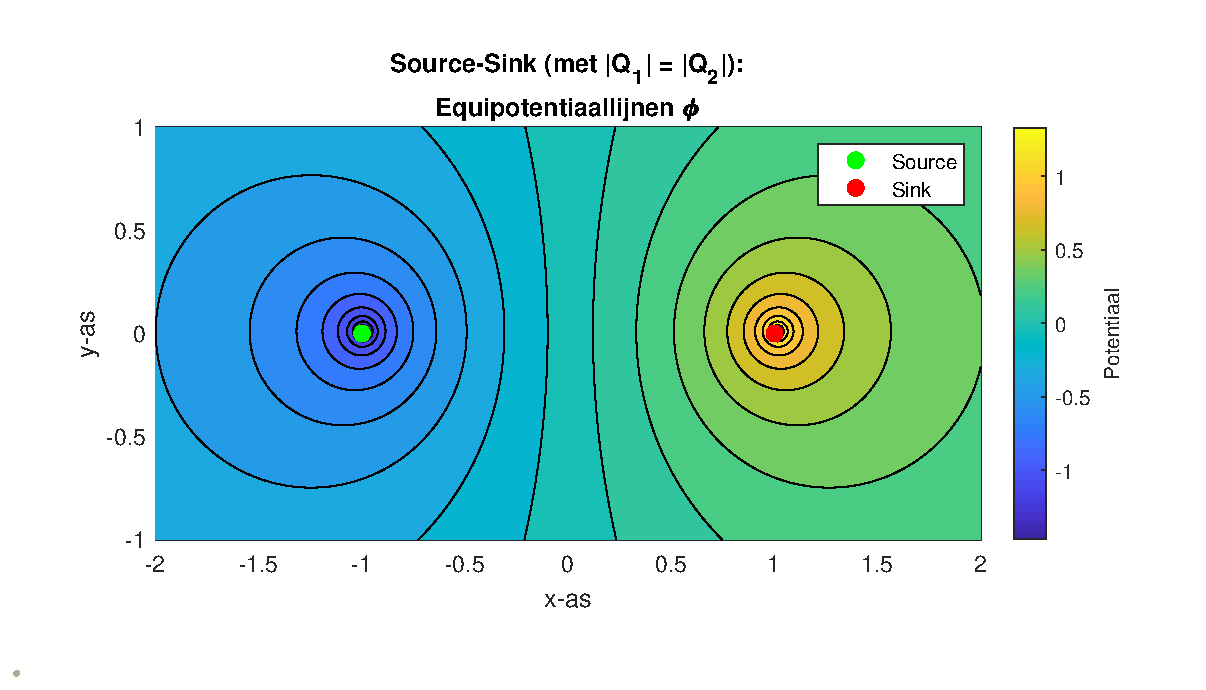
\includegraphics[width = \textwidth]{plots/probleem1_2.eps}
    \caption{Weergave van equipotentiaallijnen voor een source-sink paar.}
    \label{probleem1_2}
  \end{figure}
  \begin{figure}[ht!]
    \centering
    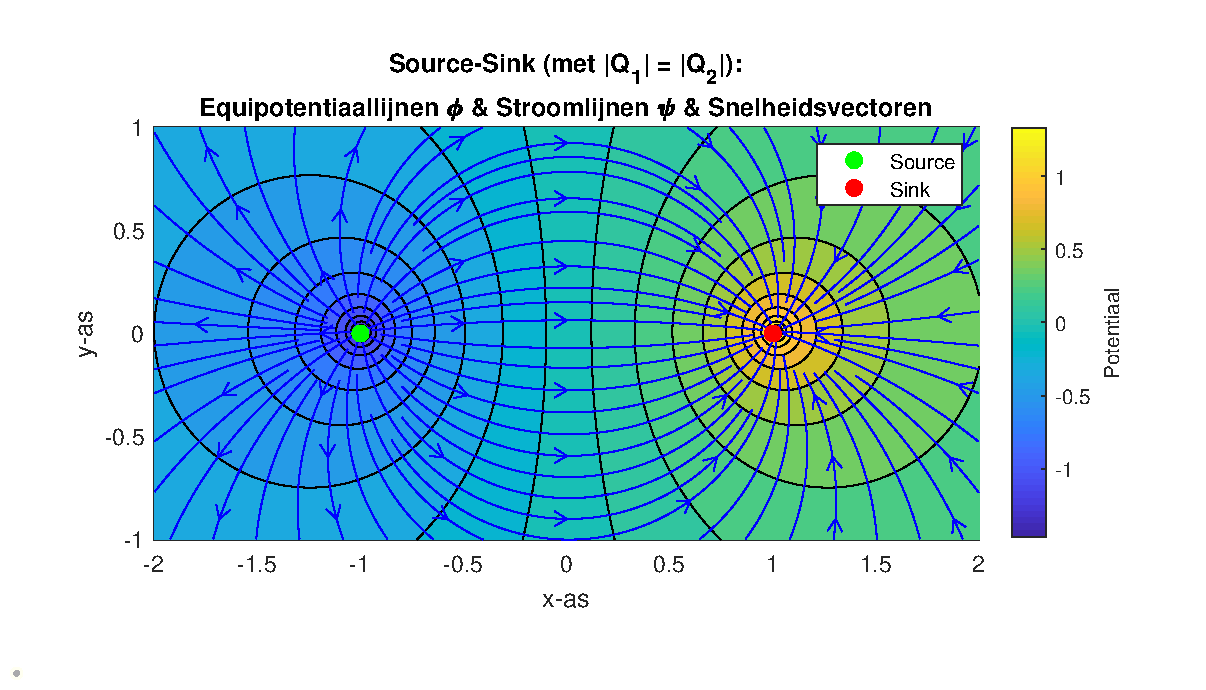
\includegraphics[width = \textwidth]{plots/probleem1_3.eps}
    \caption{Weergave van stroomlijnen, snelheidsvectoren, en equipotentiaallijnen voor een source-sink paar.}
    \label{probleem1_3}
  \end{figure}
  \begin{figure}[ht!]
    \centering
    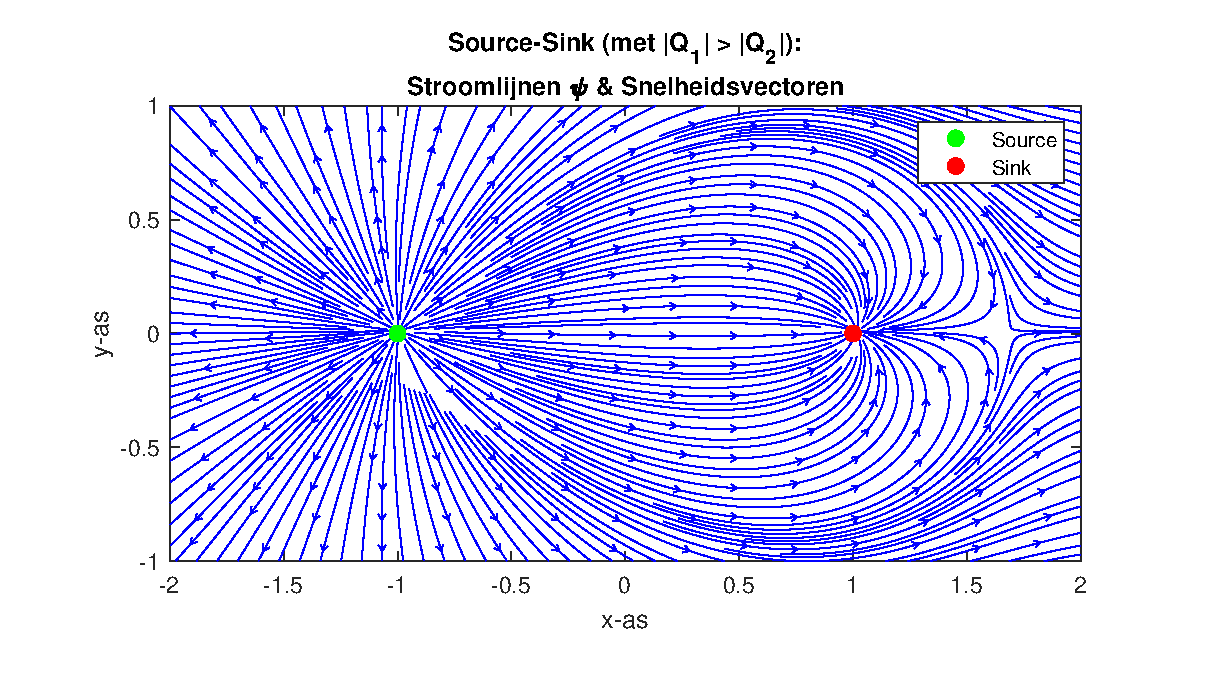
\includegraphics[width = \textwidth]{plots/probleem1_4.eps}
    \caption{Weergave van stroomlijnen en snelheidsvectoren voor een source-sink paar waarbij de source een factor 4 keer sterker is dan de sink.}
    \label{probleem1_4}
  \end{figure}
  \begin{figure}[ht!]
    \centering\vspace{-1.5cm}
    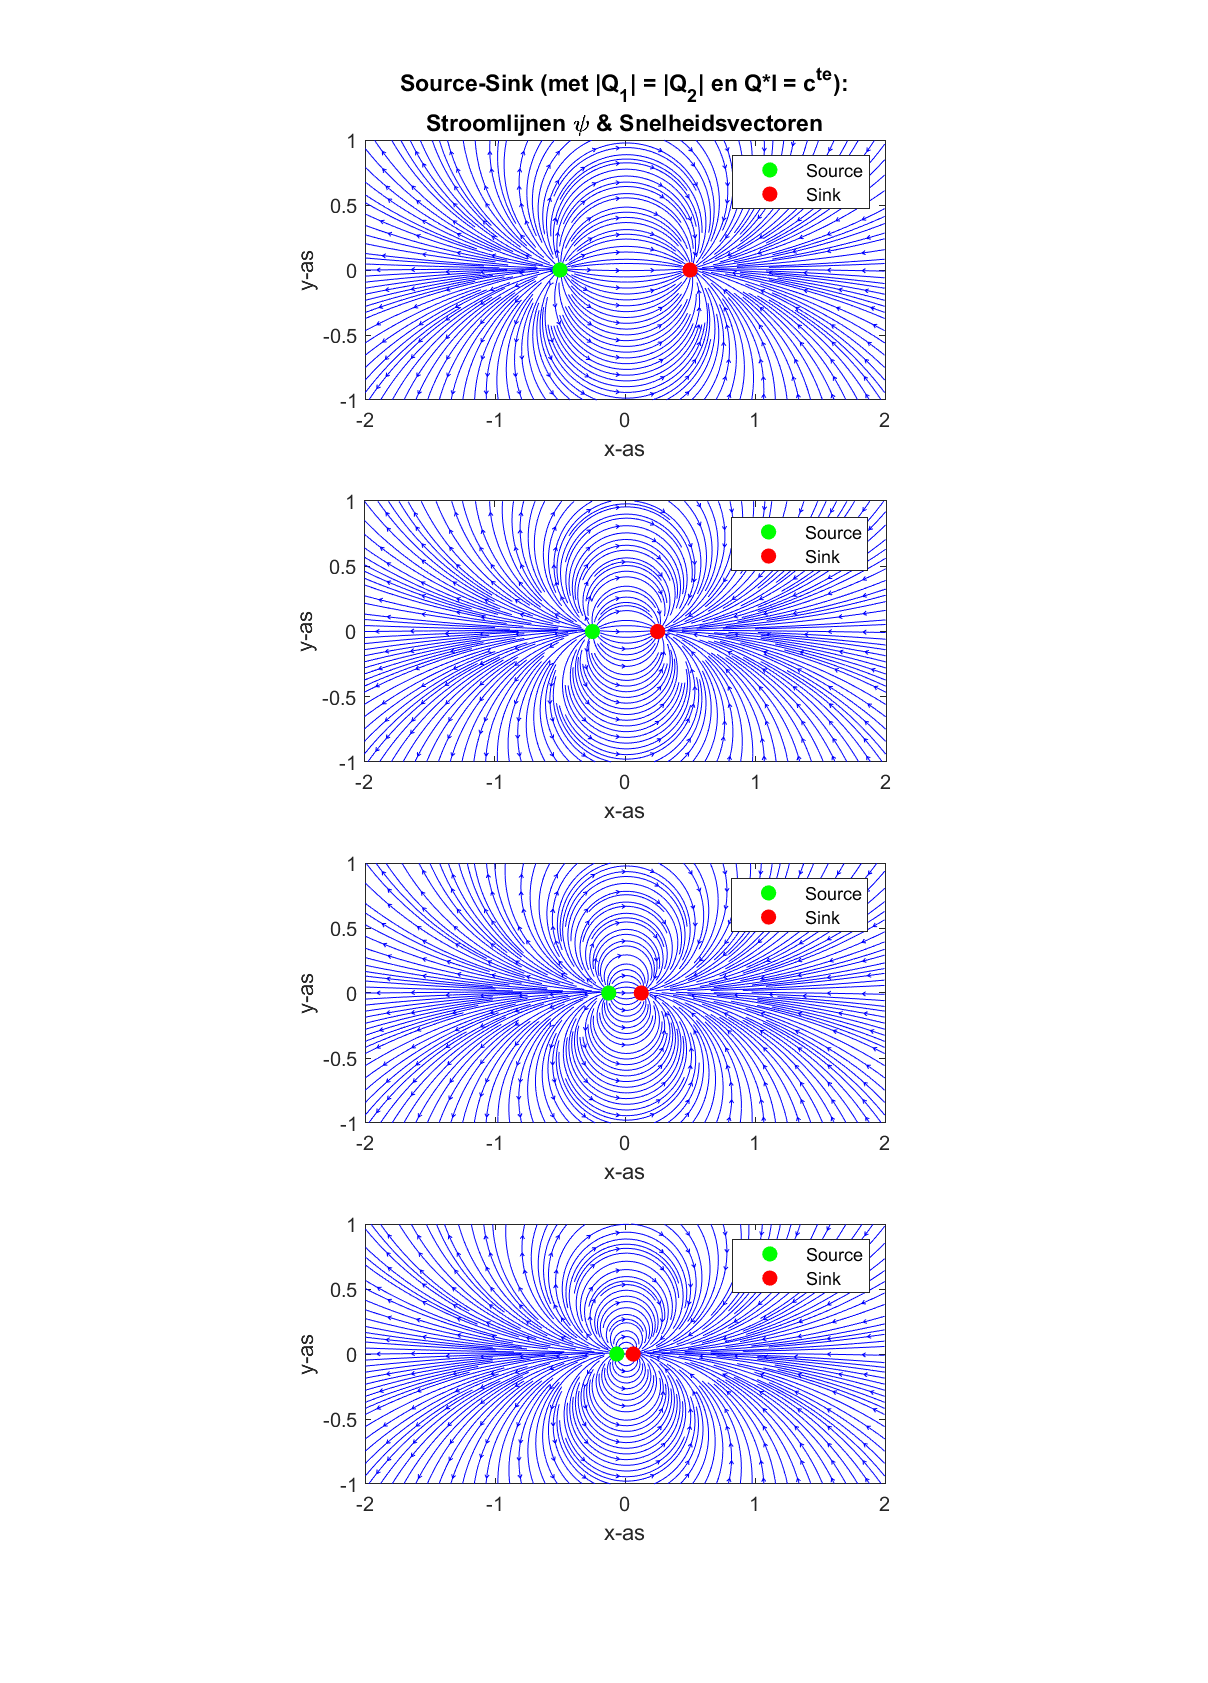
\includegraphics[width = \textwidth]{plots/probleem1_5.eps}\vspace{-1cm}
    \caption{Source-sink paar waarbij men observeert dat voor de limiet van $\ell\rightarrow0$ men een source-sink doublet bekomt, daar $Q\cdot\ell=c^{te}$.}
    \label{probleem1_5}
  \end{figure}
  \FloatBarrier

\newpage
\section{Probleem 2: Een source in uniforme stroming}
  \noindent
  In deze opdracht werden de stroomlijnen en snelheidsvectoren gevisualiseerd voor een source in een uniforme stroom. We zien op figuur \ref{probleem2_1} een vrij intu\"itief resultaat waar de uniforme stroom afgebogen wordt in de buurt van de source en daar de stroom van de source botst op de uniforme stroom vinden we een stagnatiepunt. Dit stagnatiepunt wordt gekenmerkt door $\left|\overline{v}\p{x_{stagnatie},y_{stagnatie}}\right| = 0$. We kunnen eenvoudig de formule afleiden om de positie van dit stagnatiepunt te bepalen.\\

  \noindent
  Allereerst merken we op dat het probleem translatie-invariant is langs de $y$-as voor het geval van een uniforme stroming langs de $x$-as. Er volgt dus direct dat:

  \begin{equation*}
    y_{stagnatie} = y_{source}
  \end{equation*}

  \noindent
  Dan kunnen we voor de $x$-positie van het stagnatiepunt gebruik maken van het principe van superpositie, waaruit volgt dat:

  \begin{equation*}
    \overline{v}_{totaal} = \overline{v}_{uniform} + \overline{v}_{source}
  \end{equation*}

  \noindent
  We kunnen deze vergelijking dan nog splitsen per component, gezien we al weten waar de $y$-component van het stagnatiepunt zal zijn, beschouwen we enkel de $x$-component van de vector:

  \begin{equation*}
    v_{totaal,x} = v_{uniform,x} + v_{source,x}
  \end{equation*}

  \noindent
  Uit de opdracht \cite{opdracht} weten we ook dat:

  \begin{equation*}
    \left\{
    \begin{align}
      v_{uniform,x}\p{x,y} &= U_\infty\cos\alpha \\
      v_{source,x}\p{x,y}  &= \frac{Q}{2\pi}\frac{\p{x-x_{source}}}{\p{x-x_{source}}^2+\p{y-y_{source}}^2}
    \end{align}
    \right.
  \end{equation*}

  \noindent
  Invullen dat $\alpha=0$ en optellen om $v_{totaal,x}$ te verkrijgen levert:

  \begin{equation*}
    v_{totaal,x} = U_\infty+\frac{Q}{2\pi}\frac{\p{x-x_{source}}}{\p{x-x_{source}}^2+\p{y-y_{source}}^2}
  \end{equation*}

  \noindent
  We zoeken $\p{x_{stagnatie}, y_{stagnatie}}$ opdat $v_{totaal,x} = 0$, we vullen alvast voor de $y$-waarde in dat $y = y_{stagnatie} = y_{source}$, waardoor de uitdrukking vereenvoudigt tot:

  \begin{equation*}
    0 = U_\infty+\frac{Q}{2\pi}\frac{1}{x_{stagnatie}-x_{source}}
  \end{equation*}

  \noindent
  Herschikken levert dan eenvoudigweg:

  \begin{equation*}
    x_{stagnatie} = x_{source}-\frac{Q}{2\pi U_\infty}
  \end{equation*}

\newpage
  \noindent
  Er volgt dus dat het stagnatiepunt gelegen is op de co\"ordinaat:

  \begin{equation*}
    \p{x,y} = \p{x_{source}-\frac{Q}{2\pi U_\infty}, y_{source}}
  \end{equation*}

  \noindent
  Dit kan ook met de simulatie aangetoond worden daar we op het contourplot weergegeven op figuur \ref{probleem2_2} zien dat op deze co\"ordinaat de norm van de snelheidsvector nul wordt. \\

  \noindent
  Tot slot van deze opdracht zien we ook nog op figuur \ref{probleem2_1} dat er een verdelende stroomlijn zichtbaar is langs de $x$-as voor $x\in]-\infty,x_{stagnatie}]$. Alle stroomlijnen boven deze lijn zullen langs boven over de source lopen, alle stroomlijnen hieronder zullen onder de source lopen. De halve ovaal waar de stroomlijnen van de uniforme stroom en de source elkaar ontmoeten noemt met de Rankine half body

  \FloatBarrier
  \begin{figure}[ht!]
    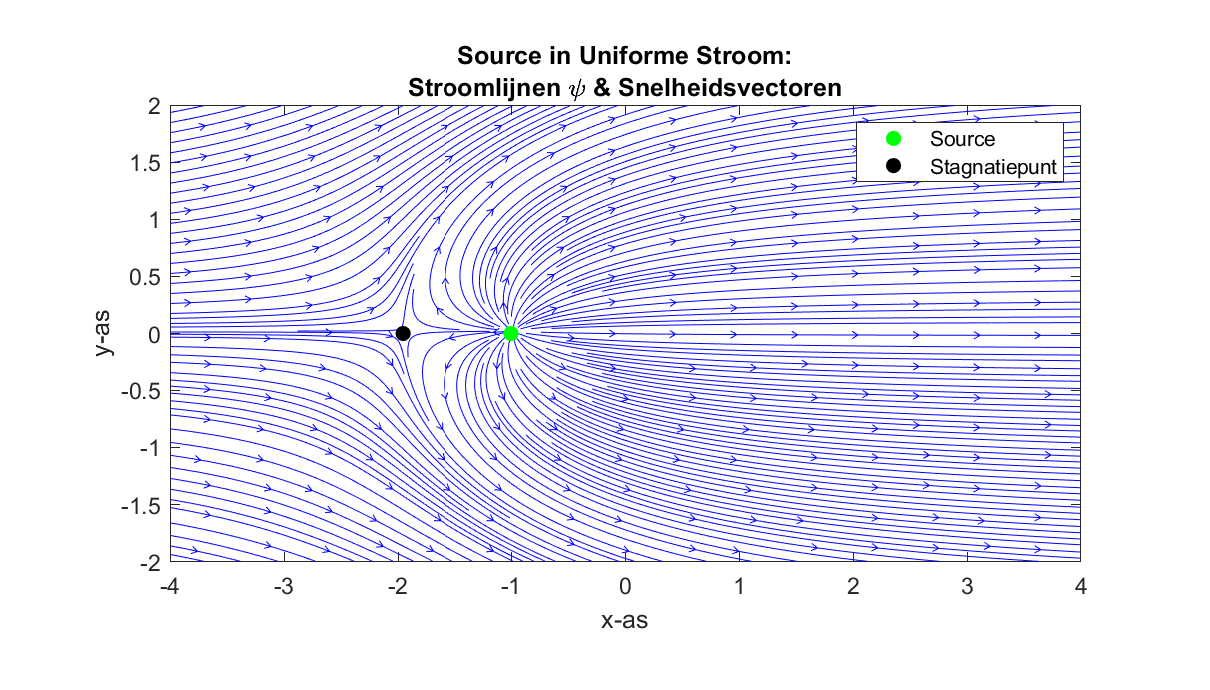
\includegraphics[width = \textwidth]{plots/probleem2_1.eps}
    \caption{Een source in uniforme stroming met stagnatiepunt en verdelende stroomlijn lopende langs de $x$-as in het domein $]-\infty,x_{stagnatie}]$.}
    \label{probleem2_1}
  \end{figure}
  \begin{figure}[ht!]
    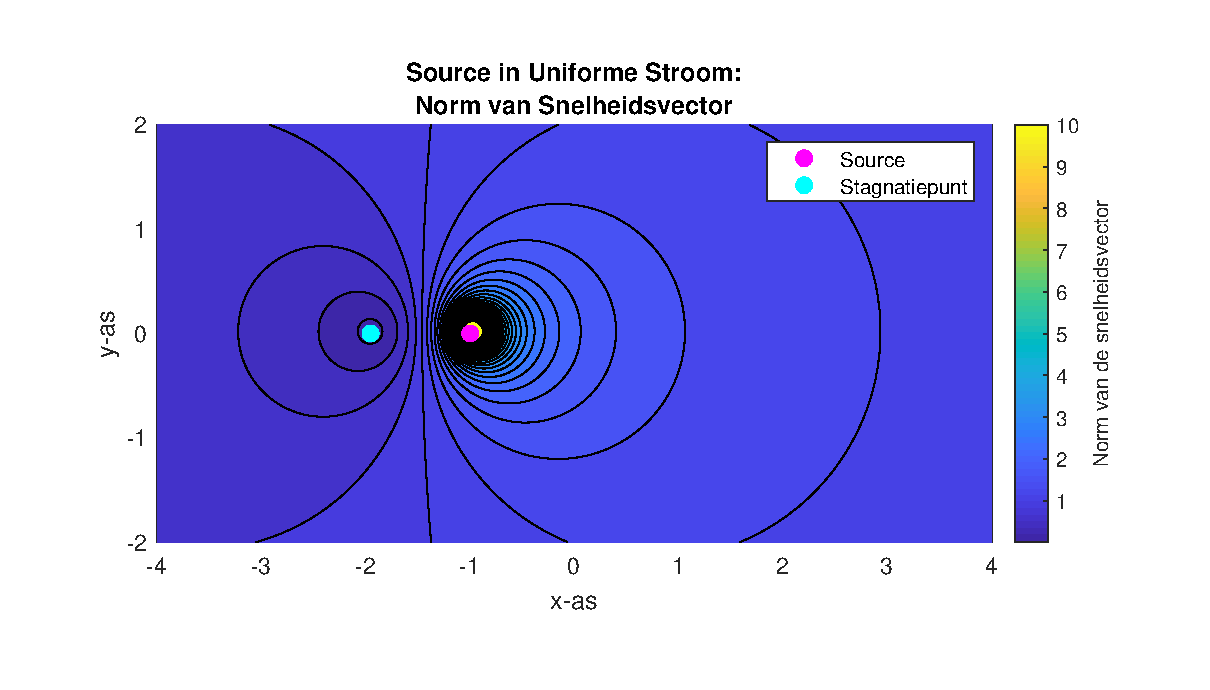
\includegraphics[width = \textwidth]{plots/probleem2_2.eps}
    \caption{Contourplot van de norm van de snelheidsvectoren.}
    \label{probleem2_2}
  \end{figure}
  \FloatBarrier

\newpage
\section{Probleem 3: Een source-sink pair in een uniform flow}
  \noindent
  ...


\newpage
\begin{thebibliography}{99}
  \bibitem{opdracht} N. van Remortel \& M. Verstraeten (2019). \textit{Examenopdracht Inleiding Programmeren: Numerieke benadering van aerodynamische problemen met behulp van potentiaalstromings theorie}, UAntwerpen.
  \bibitem{cursus} C. Beaume (ONGEKEND). \textit{Fundamentals of Fluid Mechanics}, Department of Aeronautics // Imperial College London.
\end{thebibliography}

\end{document}
